

\documentclass{article}
\usepackage[utf8]{inputenc}
\usepackage{ulem}
\usepackage[usenames]{color}
\usepackage{graphicx}


\title{	\xout{¿Cómo nos defendemos de los patógenos?} El antivirus biológico. Las células T y su comportamiento}
\author{Belén Serrano Antón }


\begin{document}
	
	\begin{titlepage}
		\maketitle
	\end{titlepage}
	
	\section{Introducción}
	\xout{La habilidad de nuestro sistema inmune para combatir patógenos, ya sean internos (como un tumor) o externos (como una infección por microbios) es ciertamente apasionante. }
	
	Como si de un campo de batalla se tratara, nuestro cuerpo es testigo de numerosas contiendas que el sistema inmune libra para mantenernos sanos. No es una tarea fácil, pues estamos continuamente expuestos a posibles atacantes.
	\\
	Sin embargo, la habilidad de nuestro sistema inmune para protegernos de los patógenos es ciertamente apasionante. Las células inmunes no solo tienen que identificar quiénes son nuestros amigos y quiénes nuestros enemigos, también tienen que saber cómo y dónde actuar.
	\\
	\\
	Si bien parece natural pensar que hay un órgano que actúa de director, ese órgano, si existe, aún no se ha encontrado. Incita, por tanto, a pensar, que las células inmunes basan su actuación en la información local que encuentran a su alrededor. Y sobre esta suposición construiremos un modelo que describa las dos actuaciones básicas, división y muerte celular, que desarrollan las células de nuestro estudio: las células T.
	
	 \section{Reconocimiento de antígenos}
	 Los antígenos pueden venir tanto del exterior, por ejemplo los microbios, como del interior, entre ellos, el crecimiento de un tumor(?). Pero antes de atacar hay que cerciorarse de quién es el enemigo. Para el sistema inmune es una gran responsabilidad, pues atacar a células equivocadas puede provocar daños irreparables, como puede ser el caso de enfermedades autoinmunes si estamos atacando a células propias.
	 \\
	 \\
	 De la misma manera que veníamos diciendo en la introducción, asumiremos que las células T toman sus decisiones basándose únicamente en información de su entorno, es decir, son ellas de manera individual las que sentencian, o no, al organismo de al lado.
	 \\
 	 \\
 	 Pero... ¿Cómo lo hacen?
 	 \\
 	 \\
 	 Las células dendríticas y los macrófagos \footnote{Dos tipos de células inmunes.} recorren el cuerpo tomando muestras de péptidos \footnote{Moléculas formadas por la unión de aminoácidos.} de los tejidos. Si estas detectan una infección incrementan su actividad fagocítica para comenzar a eliminar los primeros patógenos y, de manera simultánea, mandan señales de alerta para reclutar a otras células inmunes. Los péptidos recolectados se mandan a estructuras de membrana específicas cerca de los ganglios linfáticos.
 	 \\
 	 \\
 	 Es allí donde interactúan con las células T. Estas están dotadas de un receptor de membrana, que en lo que sigue llamaremos TCR (T Cell Receptor), a través del cual son capaces de comunicarse con el exterior y cuya estructura es tremendamente variable, pues no todos los TCR presentan la misma afinidad para un determinado antígeno.
 	 \\
 	 \\
 	 En los ganglios, las células T están ``desactivadas", en un estado naïve. Si, por el contrario, el TCR y un antígeno se encuentran se produce un proceso conocido como \textit{sinapsis inmmune} y la célula se activa, convirtiéndose en una \textit{célula efectora}, lista para combatir al antígeno.
 	 \textcolor{blue}{La diversidad estructural del TCR implica que solo una pequeña fracción de células T se activan en presencia de los antígenos que ha presentado una célula dendrítica.}
 	 \\
 	 A partir de este momento, el número de células T comienza a aumentar, pasando de unos cientos a millones en unas horas. Este proceso se conoce como \textit{clonal expansion}. De esta manera se consigue rápidamente un ejército con el que combatir al antígeno. La mayoría de ellas morirán después (apóptosis) y un pequeño porcentaje quedará como \textit{células con memoria}, que guardará información sobre el antígeno por si volviera a aparecer en un futuro combatirlo más rápidamente.
 	 \\
 	 \\
 	 Después de que la población de antígenos disminuya, el número de estas células T decrece rápidamente (\textit{clonal contraction}), aunque con retardo respecto a la desaparición del antígeno.
 	 
 	 \begin{figure}[h!]
 	 	\centering
 	 	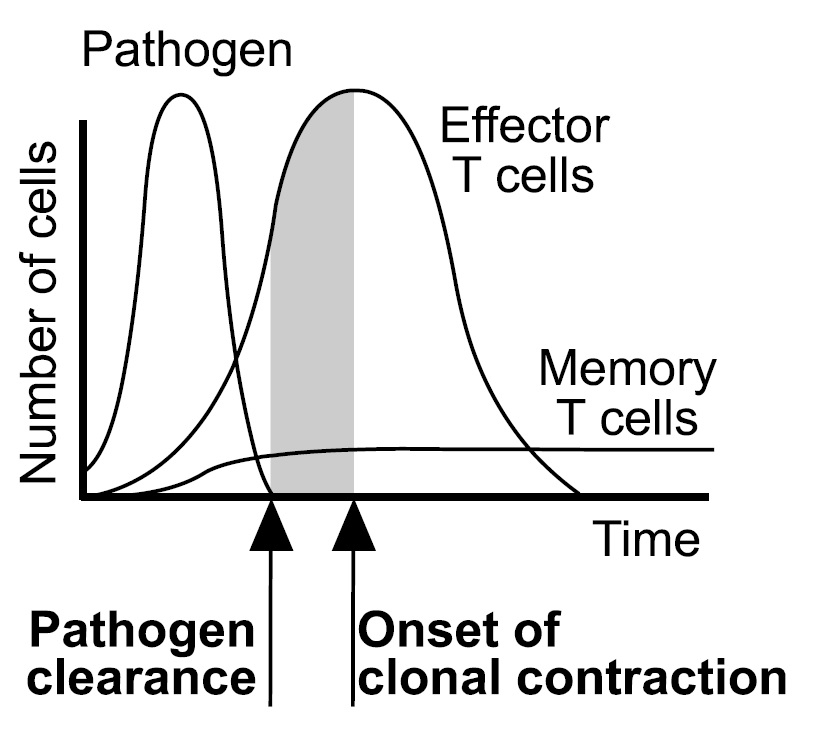
\includegraphics[width=0.4\textwidth]{clonalExpContr}
 	 	\caption{Clonal expansion/contraction}
 	 	\label{fig:ejemplo}
 	 \end{figure}
	 
	 \section{Algoritmo de decisión}
	 Todos estos cambios en el tamaño de la población (\textit{clonal expansion} y \textit{clonal contraction}), así como la diferenciación en células con memoria, puede verse de manera global como la toma de una inmensidad de decisiones individuales que hacen que todo el sistema funcione.
	 \\
	 Una vez que una célula T ha sido activada, esta puede tomar un número de opciones muy limitadas, las resumiremos en dos:
	 \begin{itemize}
	 	\item dividirse
	 	\item morir
	 \end{itemize}
     También pueden diferenciarse en células con memoria, pero trataremos este caso más adelante.
	 \\
	 \\
	 Pero, ¿qué factores afectan a esta toma de decisiones? Una primera intuición nos puede llevar a pensar que estas decisiones vienen determinadas por la presencia (o no) del antígeno. Sin embargo, sabemos que las células continúan dividiéndose aún cuando la presencia de este estímulo ya no está, o que las células cometen apóptosis aún cuando el estímulo persiste. 
	 \\
	 Siguiendo esta línea, asumiremos en nuestro modelo que estas decisiones vienen determinadas por la competición de dos moléculas inhibidoras: Retinoblastoma (Rb), que previene la expresión de genes necesarios para que la célula pueda continuar el ciclo celular y dividirse, y célula B linfoma-2 (Bcl-2), que bloqueará la muerte celular.
	 \\
	 Estableceremos que, si la cantidad de Rb cae por debajo de cierto límite, la célula T comenzará la división celular. Por el contrario, si es la cantidad de Bcl-2 la que  cae por debajo de cierto límite, provocará la apóptosis de la célula T. 
	 \\
	 \\
	 Como ya habíamos aunuciado, la célula T se comunica con el exterior gracias a su TCR, y las variaciones en la cantidad de Rb y Bcl-2 dependerán de que sean fosforiladas por unas unas moléculas llamadas citoquinas. De esta manera, la decisión de la célula T vendrá determinada por la concentración de citoquinas alrededor de ella y el número de receptores existentes en su TCR.
	\\
	Ambos procesos, división y apóptosis, son excluyentes y, en cuanto uno de ellos comienza, es interrumpible, independientemente de la acción de las citoquinas. LAS CELULAS T CON MEMORIA NO TIENEN RECEPTORES DEATH
	\\
	\\
	Con toda esta información, ya estamos en condiciones de presentar las ecuaciones de nuestro modelo: 
	\begin{itemize}
	    \item Denotaremos por \textit{$c(t)$} y \textit{$a(t)$} la cantidad de Rb y Bcl-2 activa en tiempo t, respectivamente.
	    \item \textit{$R_{i}$} será el receptor de la i-ésima citoquina y \textit{$r_{i}(t)$} será la cantidad de ese receptor en tiempo t. 
	    \item $r_{T}$ es el número de señales TCR/antíeno  percibidas por la célula T correspondiente.
	\end{itemize} 
	 Proponemos las siguientes ecuaciones diferenciales:
	 
	 \begin{displaymath}
         \left\{ \begin{array}{l}
        \dot{c}(t) = \mu_{Tc}r_{T}(t) + \sum_{j=1}^{k}\mu_{jc}r_{j}(t)\\
        \dot{a}(t) = \mu_{Ta}r_{T}(t) + \sum_{j=1}^{k}\mu_{ja}r_{j}(t) \\
        \end{array}
        \right.
    \end{displaymath}
    Estableceremos que las condiciones $a(t)=0$ y $c(t)=0$ provocarán instantáneamente la transición desde la etapa de decisión a apóptosis o división celular, respectivamente.
	\\
	Si una célula muere, será eliminada de la población. De manera contraria, si esta se divide será sustituida por dos células del mismo tipo y cuyas condiciones iniales veremos más adelante.
	\\
	\\
	La ecuación que modelará el comportamiento del TCR vendrá dada por 

	\begin{displaymath}
        \begin{array}{ll}
        \dot{r}_{i}(t) = \lambda_{Ti}r_{T}(t) + \sum_{j=1}^{k}\lambda_{ji}r_{j}(t) & \mbox{para $i=1,...,k$} 
        \end{array}
    \end{displaymath}
	En ella expresamos el carácter lineal del TCR y su dependencia de la cantidad del resto de receptores y el número de señales percibidas por la célula T. 
	\\
	Las ecuaciones que hemos tomado son lineales porque suponemos que los TCR son independientes y tienen efectos acumulativos. Así mismo, nos permiten establecer que para configuraciones de membrana similares, las células T tomarán decisiones similares.
	\\
	\\
	Nos quedaría ahora establecer qué ocurre con los TCR cuando una célula se divide. 
	\\
	Al contrario que las células T desactivadas (naïve), las células T con memoria y las células T efectoras se dividen de manera simétrica. Es decir, comparten sus receptores de membrana con sus dos células hija siguiendo la ecuación:
	
	\begin{displaymath}
         \left\{ \begin{array}{l}
        r_{i0}^{1}= \delta_{i}^{x} r_{i}^{x}\\
        r_{i0}^{2}= (1-\delta_{i}^{x}) r_{i}^{x} \\
        \end{array}
        \right.
    \end{displaymath}
	Donde $\delta_{i}^{x}$ representa el ratio de receptores de membrana de tipo $R_{i}$ entre las células hijas, $r_{i0}^{1}$ y $r_{i0}^{2}$ denotan los valores iniciales de receptor $R_{i}$ en las células hijas 1 y 2, respectivamente, y  $r_{i}^{x}$ denota el número de receptores $R_{i}$ en la célula T $x$ en el momento de la división celular.
	
	\section{Interacciones patógeno-célula T}
	Usaremos una ecuación genérica (que no se centra en un patógeno concreto) para describir las interacciones entre los patógenos y las células T.
	
	\begin{displaymath}
	\begin{array}{ll}
	\dot{y}(t) = \alpha y(t) - \beta n(t)y(t)
	\end{array}
	\end{displaymath}
	
	Donde $y(t)$ representa el número de células patógeno y $n(t)$ el número de células T en un tiempo $t$. Asumimos que estas funciones son positivas, pues no puede haber un número negativo de individuos, y que también son positivos los parámetros $\alpha$ y $\beta$ que dependerán del patógeno concreto.
	\\
	Con esta ecuación establecemos que los patógenos aumentan su población hasta que las células T superan un determinado número. Es entonces cuando el término que acompaña al parámetro $\beta$ es lo suficiente grande como para hacer decrecer la población de patógenos.
	\\
	\\
	(Lotka–Volterra predator–prey)
	
	\section{Conclusiones}
	Hemos visto un algoritmo muy simple, que modeliza las decisiones de las células T.
	\\
	A pesar de que el modelo se asemeja a lo que observamos experimentalmente, aún quedan muchas cosas por resolver, una de las más importantes es: ¿cómo puede ser que si el comportamiento de estas células depende de decisiones locales veamos un comportamiento global? Es decir, que las células T funcionen como un ``equipo" para protegernos de los patógenos. 
	
	
\end{document}